\documentclass[twoside]{book}

% Packages required by doxygen
\usepackage{fixltx2e}
\usepackage{calc}
\usepackage{doxygen}
\usepackage[export]{adjustbox} % also loads graphicx
\usepackage{graphicx}
\usepackage[utf8]{inputenc}
\usepackage{makeidx}
\usepackage{multicol}
\usepackage{multirow}
\PassOptionsToPackage{warn}{textcomp}
\usepackage{textcomp}
\usepackage[nointegrals]{wasysym}
\usepackage[table]{xcolor}

% Font selection
\usepackage[T1]{fontenc}
\usepackage[scaled=.90]{helvet}
\usepackage{courier}
\usepackage{amssymb}
\usepackage{sectsty}
\renewcommand{\familydefault}{\sfdefault}
\allsectionsfont{%
  \fontseries{bc}\selectfont%
  \color{darkgray}%
}
\renewcommand{\DoxyLabelFont}{%
  \fontseries{bc}\selectfont%
  \color{darkgray}%
}
\newcommand{\+}{\discretionary{\mbox{\scriptsize$\hookleftarrow$}}{}{}}

% Page & text layout
\usepackage{geometry}
\geometry{%
  a4paper,%
  top=2.5cm,%
  bottom=2.5cm,%
  left=2.5cm,%
  right=2.5cm%
}
\tolerance=750
\hfuzz=15pt
\hbadness=750
\setlength{\emergencystretch}{15pt}
\setlength{\parindent}{0cm}
\setlength{\parskip}{3ex plus 2ex minus 2ex}
\makeatletter
\renewcommand{\paragraph}{%
  \@startsection{paragraph}{4}{0ex}{-1.0ex}{1.0ex}{%
    \normalfont\normalsize\bfseries\SS@parafont%
  }%
}
\renewcommand{\subparagraph}{%
  \@startsection{subparagraph}{5}{0ex}{-1.0ex}{1.0ex}{%
    \normalfont\normalsize\bfseries\SS@subparafont%
  }%
}
\makeatother

% Headers & footers
\usepackage{fancyhdr}
\pagestyle{fancyplain}
\fancyhead[LE]{\fancyplain{}{\bfseries\thepage}}
\fancyhead[CE]{\fancyplain{}{}}
\fancyhead[RE]{\fancyplain{}{\bfseries\leftmark}}
\fancyhead[LO]{\fancyplain{}{\bfseries\rightmark}}
\fancyhead[CO]{\fancyplain{}{}}
\fancyhead[RO]{\fancyplain{}{\bfseries\thepage}}
\fancyfoot[LE]{\fancyplain{}{}}
\fancyfoot[CE]{\fancyplain{}{}}
\fancyfoot[RE]{\fancyplain{}{\bfseries\scriptsize Generated by Doxygen }}
\fancyfoot[LO]{\fancyplain{}{\bfseries\scriptsize Generated by Doxygen }}
\fancyfoot[CO]{\fancyplain{}{}}
\fancyfoot[RO]{\fancyplain{}{}}
\renewcommand{\footrulewidth}{0.4pt}
\renewcommand{\chaptermark}[1]{%
  \markboth{#1}{}%
}
\renewcommand{\sectionmark}[1]{%
  \markright{\thesection\ #1}%
}

% Indices & bibliography
\usepackage{natbib}
\usepackage[titles]{tocloft}
\setcounter{tocdepth}{3}
\setcounter{secnumdepth}{5}
\makeindex

% Hyperlinks (required, but should be loaded last)
\usepackage{ifpdf}
\ifpdf
  \usepackage[pdftex,pagebackref=true]{hyperref}
\else
  \usepackage[ps2pdf,pagebackref=true]{hyperref}
\fi
\hypersetup{%
  colorlinks=true,%
  linkcolor=blue,%
  citecolor=blue,%
  unicode%
}

% Custom commands
\newcommand{\clearemptydoublepage}{%
  \newpage{\pagestyle{empty}\cleardoublepage}%
}

\usepackage{caption}
\captionsetup{labelsep=space,justification=centering,font={bf},singlelinecheck=off,skip=4pt,position=top}

%===== C O N T E N T S =====

\begin{document}

% Titlepage & ToC
\hypersetup{pageanchor=false,
             bookmarksnumbered=true,
             pdfencoding=unicode
            }
\pagenumbering{roman}
\begin{titlepage}
\vspace*{7cm}
\begin{center}%
{\Large Frontier Exploration Robot }\\
\vspace*{1cm}
{\large Generated by Doxygen 1.8.11}\\
\end{center}
\end{titlepage}
\clearemptydoublepage
\tableofcontents
\clearemptydoublepage
\pagenumbering{arabic}
\hypersetup{pageanchor=true}

%--- Begin generated contents ---
\chapter{Hierarchical Index}
\section{Class Hierarchy}
This inheritance list is sorted roughly, but not completely, alphabetically\+:\begin{DoxyCompactList}
\item \contentsline{section}{Publisher\+Tests}{\pageref{classPublisherTests}}{}
\item Test\begin{DoxyCompactList}
\item \contentsline{section}{Frontier\+Explore\+Tests}{\pageref{classFrontierExploreTests}}{}
\item \contentsline{section}{Occupancy\+Map\+Tests}{\pageref{classOccupancyMapTests}}{}
\end{DoxyCompactList}
\end{DoxyCompactList}

\chapter{Class Index}
\section{Class List}
Here are the classes, structs, unions and interfaces with brief descriptions\+:\begin{DoxyCompactList}
\item\contentsline{section}{\hyperlink{classFrontierExploreTests}{Frontier\+Explore\+Tests} \\*Class \hyperlink{classOccupancyMapTests}{Occupancy\+Map\+Tests} used for setup and teardown for all the tests }{\pageref{classFrontierExploreTests}}{}
\item\contentsline{section}{\hyperlink{classOccupancyMapTests}{Occupancy\+Map\+Tests} \\*Class \hyperlink{classOccupancyMapTests}{Occupancy\+Map\+Tests} used for setup and teardown for all the tests }{\pageref{classOccupancyMapTests}}{}
\item\contentsline{section}{\hyperlink{classPublisherTests}{Publisher\+Tests} \\*Class \hyperlink{classPublisherTests}{Publisher\+Tests} used for testing publisher }{\pageref{classPublisherTests}}{}
\end{DoxyCompactList}

\chapter{File Index}
\section{File List}
Here is a list of all documented files with brief descriptions\+:\begin{DoxyCompactList}
\item\contentsline{section}{/home/rohith/1808push/src/frontier\+\_\+exploration/src/\hyperlink{frontier__exploration__node_8cpp}{frontier\+\_\+exploration\+\_\+node.\+cpp} \\*Source file for Frontier\+Explore class }{\pageref{frontier__exploration__node_8cpp}}{}
\item\contentsline{section}{/home/rohith/1808push/src/frontier\+\_\+exploration/src/\hyperlink{map__structure_8cpp}{map\+\_\+structure.\+cpp} \\*Source file for Map\+Structure class }{\pageref{map__structure_8cpp}}{}
\item\contentsline{section}{/home/rohith/1808push/src/frontier\+\_\+exploration/src/\hyperlink{occupancy__map_8cpp}{occupancy\+\_\+map.\+cpp} \\*Source file for Occupancy\+Map class }{\pageref{occupancy__map_8cpp}}{}
\item\contentsline{section}{/home/rohith/1808push/src/frontier\+\_\+exploration/test/\hyperlink{frontier__exploration__node__tests_8cpp}{frontier\+\_\+exploration\+\_\+node\+\_\+tests.\+cpp} \\*Source file for testing Map\+Structure class }{\pageref{frontier__exploration__node__tests_8cpp}}{}
\item\contentsline{section}{/home/rohith/1808push/src/frontier\+\_\+exploration/test/\hyperlink{map__structure__tests_8cpp}{map\+\_\+structure\+\_\+tests.\+cpp} \\*Source file for testing Map\+Structure class }{\pageref{map__structure__tests_8cpp}}{}
\item\contentsline{section}{/home/rohith/1808push/src/frontier\+\_\+exploration/test/\hyperlink{occupancy__map__tests_8cpp}{occupancy\+\_\+map\+\_\+tests.\+cpp} \\*Source file for testing Occupancy\+Map class }{\pageref{occupancy__map__tests_8cpp}}{}
\end{DoxyCompactList}

\chapter{Class Documentation}
\hypertarget{classFrontierExploreTests}{}\section{Frontier\+Explore\+Tests Class Reference}
\label{classFrontierExploreTests}\index{Frontier\+Explore\+Tests@{Frontier\+Explore\+Tests}}


class \hyperlink{classOccupancyMapTests}{Occupancy\+Map\+Tests} used for setup and teardown for all the tests  




Inheritance diagram for Frontier\+Explore\+Tests\+:
\nopagebreak
\begin{figure}[H]
\begin{center}
\leavevmode
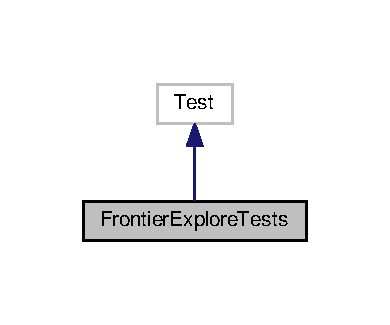
\includegraphics[width=187pt]{classFrontierExploreTests__inherit__graph}
\end{center}
\end{figure}


Collaboration diagram for Frontier\+Explore\+Tests\+:
\nopagebreak
\begin{figure}[H]
\begin{center}
\leavevmode
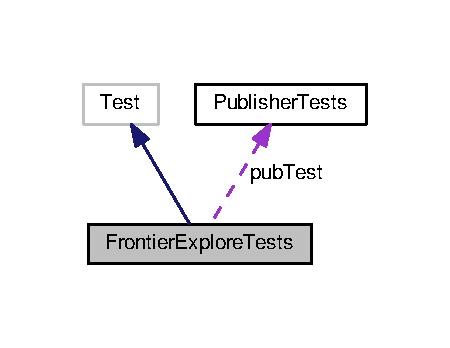
\includegraphics[width=216pt]{classFrontierExploreTests__coll__graph}
\end{center}
\end{figure}
\subsection*{Public Member Functions}
\begin{DoxyCompactItemize}
\item 
\hyperlink{classFrontierExploreTests_a3033043f511d924f988782a3a802f63e}{Frontier\+Explore\+Tests} ()
\begin{DoxyCompactList}\small\item\em Default constructor for \hyperlink{classFrontierExploreTests}{Frontier\+Explore\+Tests}. \end{DoxyCompactList}\item 
\hyperlink{classFrontierExploreTests_a7cb89f2326e1501e8879a7fdc5581d4c}{$\sim$\+Frontier\+Explore\+Tests} ()
\begin{DoxyCompactList}\small\item\em Default destructor for \hyperlink{classFrontierExploreTests}{Frontier\+Explore\+Tests}. \end{DoxyCompactList}\item 
void \hyperlink{classFrontierExploreTests_a8ffa7be235a89d196f8a0ab569838966}{Set\+Up} ()
\begin{DoxyCompactList}\small\item\em setup up function to set up the tests with variables or objects \end{DoxyCompactList}\item 
void \hyperlink{classFrontierExploreTests_a868ce040cbbb4ca5f1ad2573f43f4b22}{Tear\+Down} ()
\begin{DoxyCompactList}\small\item\em tear down function for the tests to clear up the used variables or objects \end{DoxyCompactList}\end{DoxyCompactItemize}
\subsection*{Public Attributes}
\begin{DoxyCompactItemize}
\item 
ros\+::\+Node\+Handle {\bfseries testnh}\hypertarget{classFrontierExploreTests_a0684ad7e48d96d232fad6b4294938f60}{}\label{classFrontierExploreTests_a0684ad7e48d96d232fad6b4294938f60}

\item 
Frontier\+Explore {\bfseries test\+Bot}\hypertarget{classFrontierExploreTests_ac738c36e2f8b1a633167b8ca0afd2626}{}\label{classFrontierExploreTests_ac738c36e2f8b1a633167b8ca0afd2626}

\item 
\hyperlink{classPublisherTests}{Publisher\+Tests} {\bfseries pub\+Test}\hypertarget{classFrontierExploreTests_a24f2d818efe00a4566fd50c9f3d18a15}{}\label{classFrontierExploreTests_a24f2d818efe00a4566fd50c9f3d18a15}

\end{DoxyCompactItemize}


\subsection{Detailed Description}
class \hyperlink{classOccupancyMapTests}{Occupancy\+Map\+Tests} used for setup and teardown for all the tests 

\subsection{Constructor \& Destructor Documentation}
\index{Frontier\+Explore\+Tests@{Frontier\+Explore\+Tests}!Frontier\+Explore\+Tests@{Frontier\+Explore\+Tests}}
\index{Frontier\+Explore\+Tests@{Frontier\+Explore\+Tests}!Frontier\+Explore\+Tests@{Frontier\+Explore\+Tests}}
\subsubsection[{\texorpdfstring{Frontier\+Explore\+Tests()}{FrontierExploreTests()}}]{\setlength{\rightskip}{0pt plus 5cm}Frontier\+Explore\+Tests\+::\+Frontier\+Explore\+Tests (
\begin{DoxyParamCaption}
{}
\end{DoxyParamCaption}
)\hspace{0.3cm}{\ttfamily [inline]}}\hypertarget{classFrontierExploreTests_a3033043f511d924f988782a3a802f63e}{}\label{classFrontierExploreTests_a3033043f511d924f988782a3a802f63e}


Default constructor for \hyperlink{classFrontierExploreTests}{Frontier\+Explore\+Tests}. 


\begin{DoxyParams}{Parameters}
{\em nothing} & \\
\hline
\end{DoxyParams}
\begin{DoxyReturn}{Returns}
nothing 
\end{DoxyReturn}
\index{Frontier\+Explore\+Tests@{Frontier\+Explore\+Tests}!````~Frontier\+Explore\+Tests@{$\sim$\+Frontier\+Explore\+Tests}}
\index{````~Frontier\+Explore\+Tests@{$\sim$\+Frontier\+Explore\+Tests}!Frontier\+Explore\+Tests@{Frontier\+Explore\+Tests}}
\subsubsection[{\texorpdfstring{$\sim$\+Frontier\+Explore\+Tests()}{~FrontierExploreTests()}}]{\setlength{\rightskip}{0pt plus 5cm}Frontier\+Explore\+Tests\+::$\sim$\+Frontier\+Explore\+Tests (
\begin{DoxyParamCaption}
{}
\end{DoxyParamCaption}
)\hspace{0.3cm}{\ttfamily [inline]}}\hypertarget{classFrontierExploreTests_a7cb89f2326e1501e8879a7fdc5581d4c}{}\label{classFrontierExploreTests_a7cb89f2326e1501e8879a7fdc5581d4c}


Default destructor for \hyperlink{classFrontierExploreTests}{Frontier\+Explore\+Tests}. 


\begin{DoxyParams}{Parameters}
{\em nothing} & \\
\hline
\end{DoxyParams}
\begin{DoxyReturn}{Returns}
nothing 
\end{DoxyReturn}


\subsection{Member Function Documentation}
\index{Frontier\+Explore\+Tests@{Frontier\+Explore\+Tests}!Set\+Up@{Set\+Up}}
\index{Set\+Up@{Set\+Up}!Frontier\+Explore\+Tests@{Frontier\+Explore\+Tests}}
\subsubsection[{\texorpdfstring{Set\+Up()}{SetUp()}}]{\setlength{\rightskip}{0pt plus 5cm}void Frontier\+Explore\+Tests\+::\+Set\+Up (
\begin{DoxyParamCaption}
{}
\end{DoxyParamCaption}
)\hspace{0.3cm}{\ttfamily [inline]}}\hypertarget{classFrontierExploreTests_a8ffa7be235a89d196f8a0ab569838966}{}\label{classFrontierExploreTests_a8ffa7be235a89d196f8a0ab569838966}


setup up function to set up the tests with variables or objects 


\begin{DoxyParams}{Parameters}
{\em nothing} & \\
\hline
\end{DoxyParams}
\begin{DoxyReturn}{Returns}
nothing 
\end{DoxyReturn}
\index{Frontier\+Explore\+Tests@{Frontier\+Explore\+Tests}!Tear\+Down@{Tear\+Down}}
\index{Tear\+Down@{Tear\+Down}!Frontier\+Explore\+Tests@{Frontier\+Explore\+Tests}}
\subsubsection[{\texorpdfstring{Tear\+Down()}{TearDown()}}]{\setlength{\rightskip}{0pt plus 5cm}void Frontier\+Explore\+Tests\+::\+Tear\+Down (
\begin{DoxyParamCaption}
{}
\end{DoxyParamCaption}
)\hspace{0.3cm}{\ttfamily [inline]}}\hypertarget{classFrontierExploreTests_a868ce040cbbb4ca5f1ad2573f43f4b22}{}\label{classFrontierExploreTests_a868ce040cbbb4ca5f1ad2573f43f4b22}


tear down function for the tests to clear up the used variables or objects 


\begin{DoxyParams}{Parameters}
{\em nothing} & \\
\hline
\end{DoxyParams}
\begin{DoxyReturn}{Returns}
nothing 
\end{DoxyReturn}


The documentation for this class was generated from the following file\+:\begin{DoxyCompactItemize}
\item 
/home/rohith/1808push/src/frontier\+\_\+exploration/test/\hyperlink{frontier__exploration__node__tests_8cpp}{frontier\+\_\+exploration\+\_\+node\+\_\+tests.\+cpp}\end{DoxyCompactItemize}

\hypertarget{classOccupancyMapTests}{}\section{Occupancy\+Map\+Tests Class Reference}
\label{classOccupancyMapTests}\index{Occupancy\+Map\+Tests@{Occupancy\+Map\+Tests}}


class \hyperlink{classOccupancyMapTests}{Occupancy\+Map\+Tests} used for setup and teardown for all the tests  




Inheritance diagram for Occupancy\+Map\+Tests\+:
\nopagebreak
\begin{figure}[H]
\begin{center}
\leavevmode
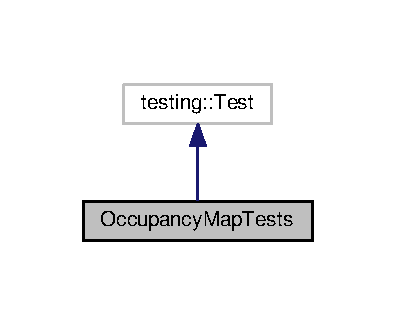
\includegraphics[width=190pt]{classOccupancyMapTests__inherit__graph}
\end{center}
\end{figure}


Collaboration diagram for Occupancy\+Map\+Tests\+:
\nopagebreak
\begin{figure}[H]
\begin{center}
\leavevmode
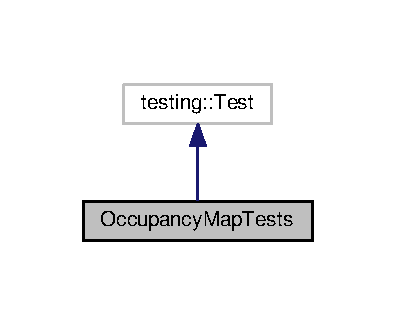
\includegraphics[width=190pt]{classOccupancyMapTests__coll__graph}
\end{center}
\end{figure}
\subsection*{Public Member Functions}
\begin{DoxyCompactItemize}
\item 
\hyperlink{classOccupancyMapTests_a50884cb585e62918588e36a80e0c768d}{Occupancy\+Map\+Tests} ()
\begin{DoxyCompactList}\small\item\em Default constructor for \hyperlink{classOccupancyMapTests}{Occupancy\+Map\+Tests}. \end{DoxyCompactList}\item 
\hyperlink{classOccupancyMapTests_ad9eecc1447f3238ba41c0cf30d865a82}{$\sim$\+Occupancy\+Map\+Tests} ()
\begin{DoxyCompactList}\small\item\em Default destructor for \hyperlink{classOccupancyMapTests}{Occupancy\+Map\+Tests}. \end{DoxyCompactList}\item 
void \hyperlink{classOccupancyMapTests_adbc4a2d53512b953005c64236de293b4}{Set\+Up} ()
\begin{DoxyCompactList}\small\item\em setup up function to set up the tests with variables or objects \end{DoxyCompactList}\item 
void \hyperlink{classOccupancyMapTests_a2fb286097387c627a3ab9c014e650d13}{Tear\+Down} ()
\begin{DoxyCompactList}\small\item\em tear down function for the tests to clear up the used variables or objects \end{DoxyCompactList}\end{DoxyCompactItemize}
\subsection*{Public Attributes}
\begin{DoxyCompactItemize}
\item 
Occupancy\+Map {\bfseries class\+Tests}\hypertarget{classOccupancyMapTests_ae95a87c63db4005c7c98c25dcee513c0}{}\label{classOccupancyMapTests_ae95a87c63db4005c7c98c25dcee513c0}

\item 
nav\+\_\+msgs\+::\+Map\+Meta\+Data {\bfseries info}\hypertarget{classOccupancyMapTests_a9356aeecd67cfffbb65a0b2c48d3b493}{}\label{classOccupancyMapTests_a9356aeecd67cfffbb65a0b2c48d3b493}

\end{DoxyCompactItemize}


\subsection{Detailed Description}
class \hyperlink{classOccupancyMapTests}{Occupancy\+Map\+Tests} used for setup and teardown for all the tests 

\subsection{Constructor \& Destructor Documentation}
\index{Occupancy\+Map\+Tests@{Occupancy\+Map\+Tests}!Occupancy\+Map\+Tests@{Occupancy\+Map\+Tests}}
\index{Occupancy\+Map\+Tests@{Occupancy\+Map\+Tests}!Occupancy\+Map\+Tests@{Occupancy\+Map\+Tests}}
\subsubsection[{\texorpdfstring{Occupancy\+Map\+Tests()}{OccupancyMapTests()}}]{\setlength{\rightskip}{0pt plus 5cm}Occupancy\+Map\+Tests\+::\+Occupancy\+Map\+Tests (
\begin{DoxyParamCaption}
{}
\end{DoxyParamCaption}
)\hspace{0.3cm}{\ttfamily [inline]}}\hypertarget{classOccupancyMapTests_a50884cb585e62918588e36a80e0c768d}{}\label{classOccupancyMapTests_a50884cb585e62918588e36a80e0c768d}


Default constructor for \hyperlink{classOccupancyMapTests}{Occupancy\+Map\+Tests}. 


\begin{DoxyParams}{Parameters}
{\em nothing} & \\
\hline
\end{DoxyParams}
\begin{DoxyReturn}{Returns}
nothing 
\end{DoxyReturn}
\index{Occupancy\+Map\+Tests@{Occupancy\+Map\+Tests}!````~Occupancy\+Map\+Tests@{$\sim$\+Occupancy\+Map\+Tests}}
\index{````~Occupancy\+Map\+Tests@{$\sim$\+Occupancy\+Map\+Tests}!Occupancy\+Map\+Tests@{Occupancy\+Map\+Tests}}
\subsubsection[{\texorpdfstring{$\sim$\+Occupancy\+Map\+Tests()}{~OccupancyMapTests()}}]{\setlength{\rightskip}{0pt plus 5cm}Occupancy\+Map\+Tests\+::$\sim$\+Occupancy\+Map\+Tests (
\begin{DoxyParamCaption}
{}
\end{DoxyParamCaption}
)\hspace{0.3cm}{\ttfamily [inline]}}\hypertarget{classOccupancyMapTests_ad9eecc1447f3238ba41c0cf30d865a82}{}\label{classOccupancyMapTests_ad9eecc1447f3238ba41c0cf30d865a82}


Default destructor for \hyperlink{classOccupancyMapTests}{Occupancy\+Map\+Tests}. 


\begin{DoxyParams}{Parameters}
{\em nothing} & \\
\hline
\end{DoxyParams}
\begin{DoxyReturn}{Returns}
nothing 
\end{DoxyReturn}


\subsection{Member Function Documentation}
\index{Occupancy\+Map\+Tests@{Occupancy\+Map\+Tests}!Set\+Up@{Set\+Up}}
\index{Set\+Up@{Set\+Up}!Occupancy\+Map\+Tests@{Occupancy\+Map\+Tests}}
\subsubsection[{\texorpdfstring{Set\+Up()}{SetUp()}}]{\setlength{\rightskip}{0pt plus 5cm}void Occupancy\+Map\+Tests\+::\+Set\+Up (
\begin{DoxyParamCaption}
{}
\end{DoxyParamCaption}
)\hspace{0.3cm}{\ttfamily [inline]}}\hypertarget{classOccupancyMapTests_adbc4a2d53512b953005c64236de293b4}{}\label{classOccupancyMapTests_adbc4a2d53512b953005c64236de293b4}


setup up function to set up the tests with variables or objects 


\begin{DoxyParams}{Parameters}
{\em nothing} & \\
\hline
\end{DoxyParams}
\begin{DoxyReturn}{Returns}
nothing 
\end{DoxyReturn}
\index{Occupancy\+Map\+Tests@{Occupancy\+Map\+Tests}!Tear\+Down@{Tear\+Down}}
\index{Tear\+Down@{Tear\+Down}!Occupancy\+Map\+Tests@{Occupancy\+Map\+Tests}}
\subsubsection[{\texorpdfstring{Tear\+Down()}{TearDown()}}]{\setlength{\rightskip}{0pt plus 5cm}void Occupancy\+Map\+Tests\+::\+Tear\+Down (
\begin{DoxyParamCaption}
{}
\end{DoxyParamCaption}
)\hspace{0.3cm}{\ttfamily [inline]}}\hypertarget{classOccupancyMapTests_a2fb286097387c627a3ab9c014e650d13}{}\label{classOccupancyMapTests_a2fb286097387c627a3ab9c014e650d13}


tear down function for the tests to clear up the used variables or objects 


\begin{DoxyParams}{Parameters}
{\em nothing} & \\
\hline
\end{DoxyParams}
\begin{DoxyReturn}{Returns}
nothing 
\end{DoxyReturn}


The documentation for this class was generated from the following file\+:\begin{DoxyCompactItemize}
\item 
/home/rohith/1808push/src/frontier\+\_\+exploration/test/\hyperlink{occupancy__map__tests_8cpp}{occupancy\+\_\+map\+\_\+tests.\+cpp}\end{DoxyCompactItemize}

\hypertarget{classPublisherTests}{}\section{Publisher\+Tests Class Reference}
\label{classPublisherTests}\index{Publisher\+Tests@{Publisher\+Tests}}


class \hyperlink{classPublisherTests}{Publisher\+Tests} used for testing publisher  


\subsection*{Public Member Functions}
\begin{DoxyCompactItemize}
\item 
void {\bfseries vel\+\_\+\+Tester} (const geometry\+\_\+msgs\+::\+Twist\+::\+Const\+Ptr \&vel\+\_\+)\hypertarget{classPublisherTests_a6dd0632aa316a9a5ee5be6063dd13608}{}\label{classPublisherTests_a6dd0632aa316a9a5ee5be6063dd13608}

\end{DoxyCompactItemize}


\subsection{Detailed Description}
class \hyperlink{classPublisherTests}{Publisher\+Tests} used for testing publisher 

The documentation for this class was generated from the following file\+:\begin{DoxyCompactItemize}
\item 
/home/rohith/1808push/src/frontier\+\_\+exploration/test/\hyperlink{frontier__exploration__node__tests_8cpp}{frontier\+\_\+exploration\+\_\+node\+\_\+tests.\+cpp}\end{DoxyCompactItemize}

\chapter{File Documentation}
\hypertarget{frontier__exploration__node_8cpp}{}\section{/home/rohith/1808push/src/frontier\+\_\+exploration/src/frontier\+\_\+exploration\+\_\+node.cpp File Reference}
\label{frontier__exploration__node_8cpp}\index{/home/rohith/1808push/src/frontier\+\_\+exploration/src/frontier\+\_\+exploration\+\_\+node.\+cpp@{/home/rohith/1808push/src/frontier\+\_\+exploration/src/frontier\+\_\+exploration\+\_\+node.\+cpp}}


source file for Frontier\+Explore class  


{\ttfamily \#include \char`\"{}frontier\+\_\+exploration\+\_\+node.\+hpp\char`\"{}}\\*
{\ttfamily \#include $<$cstdint$>$}\\*
{\ttfamily \#include $<$utility$>$}\\*
{\ttfamily \#include $<$vector$>$}\\*
{\ttfamily \#include $<$boost/range/irange.\+hpp$>$}\\*
{\ttfamily \#include \char`\"{}occupancy\+\_\+map.\+hpp\char`\"{}}\\*
{\ttfamily \#include \char`\"{}actionlib/client/simple\+\_\+action\+\_\+client.\+h\char`\"{}}\\*
{\ttfamily \#include \char`\"{}geometry\+\_\+msgs/\+Pose\+Stamped.\+h\char`\"{}}\\*
{\ttfamily \#include \char`\"{}geometry\+\_\+msgs/\+Twist.\+h\char`\"{}}\\*
{\ttfamily \#include \char`\"{}move\+\_\+base\+\_\+msgs/\+Move\+Base\+Action.\+h\char`\"{}}\\*
{\ttfamily \#include \char`\"{}nav\+\_\+msgs/\+Occupancy\+Grid.\+h\char`\"{}}\\*
{\ttfamily \#include \char`\"{}nav\+\_\+msgs/\+Odometry.\+h\char`\"{}}\\*
{\ttfamily \#include \char`\"{}ros/ros.\+h\char`\"{}}\\*
{\ttfamily \#include \char`\"{}tf/transform\+\_\+listener.\+h\char`\"{}}\\*
Include dependency graph for frontier\+\_\+exploration\+\_\+node.\+cpp\+:
\nopagebreak
\begin{figure}[H]
\begin{center}
\leavevmode
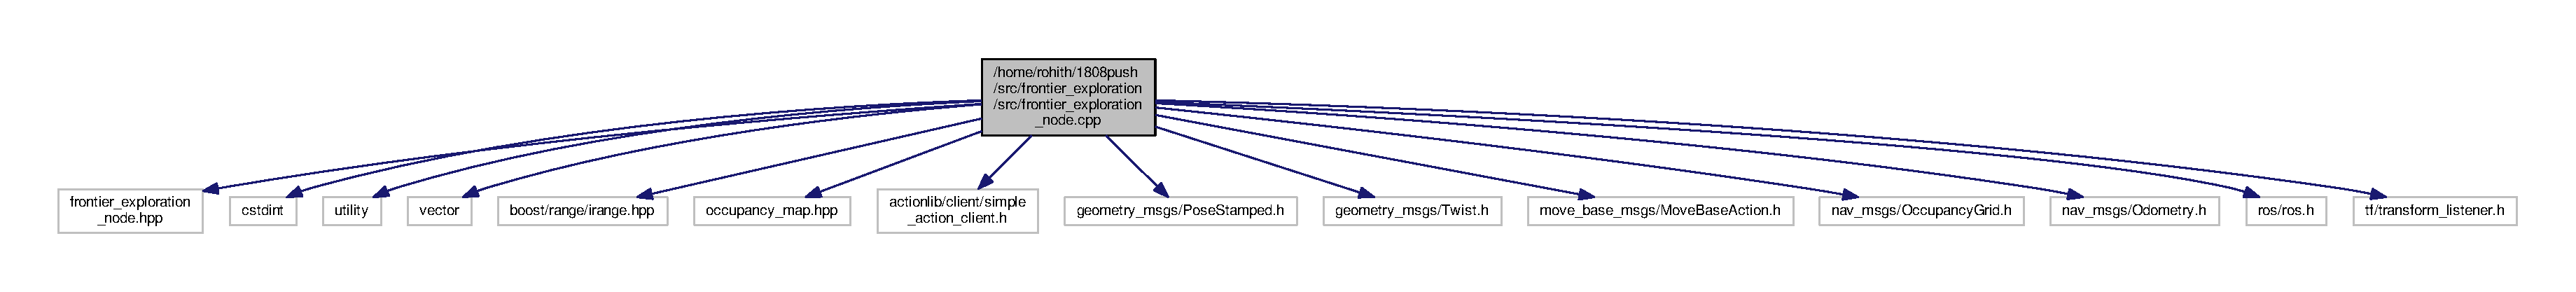
\includegraphics[width=350pt]{frontier__exploration__node_8cpp__incl}
\end{center}
\end{figure}


\subsection{Detailed Description}
source file for Frontier\+Explore class 

\begin{DoxyAuthor}{Author}
rohithjayarajan 
\end{DoxyAuthor}
\begin{DoxyDate}{Date}
16/2/2018 
\end{DoxyDate}
\begin{DoxyVersion}{Version}
1.\+1
\end{DoxyVersion}
\hypertarget{occupancy__map__tests_8cpp_DESCRIPTION}{}\subsection{D\+E\+S\+C\+R\+I\+P\+T\+I\+ON}\label{occupancy__map__tests_8cpp_DESCRIPTION}
source file which contains the defintion of Frontier\+Explore class 
\hypertarget{map__structure_8cpp}{}\section{/home/rohith/1808push/src/frontier\+\_\+exploration/src/map\+\_\+structure.cpp File Reference}
\label{map__structure_8cpp}\index{/home/rohith/1808push/src/frontier\+\_\+exploration/src/map\+\_\+structure.\+cpp@{/home/rohith/1808push/src/frontier\+\_\+exploration/src/map\+\_\+structure.\+cpp}}


source file for Map\+Structure class  


{\ttfamily \#include \char`\"{}map\+\_\+structure.\+hpp\char`\"{}}\\*
{\ttfamily \#include $<$cstdint$>$}\\*
{\ttfamily \#include $<$utility$>$}\\*
Include dependency graph for map\+\_\+structure.\+cpp\+:
\nopagebreak
\begin{figure}[H]
\begin{center}
\leavevmode
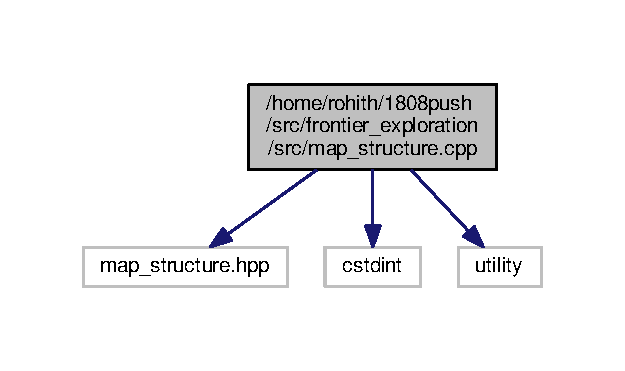
\includegraphics[width=300pt]{map__structure_8cpp__incl}
\end{center}
\end{figure}


\subsection{Detailed Description}
source file for Map\+Structure class 

\begin{DoxyAuthor}{Author}
rohithjayarajan 
\end{DoxyAuthor}
\begin{DoxyDate}{Date}
16/2/2018 
\end{DoxyDate}
\begin{DoxyVersion}{Version}
1.\+1
\end{DoxyVersion}
\hypertarget{occupancy__map__tests_8cpp_DESCRIPTION}{}\subsection{D\+E\+S\+C\+R\+I\+P\+T\+I\+ON}\label{occupancy__map__tests_8cpp_DESCRIPTION}
source file which contains the defintion of Map\+Structure class 
\hypertarget{occupancy__map_8cpp}{}\section{/home/rohith/1808push/src/frontier\+\_\+exploration/src/occupancy\+\_\+map.cpp File Reference}
\label{occupancy__map_8cpp}\index{/home/rohith/1808push/src/frontier\+\_\+exploration/src/occupancy\+\_\+map.\+cpp@{/home/rohith/1808push/src/frontier\+\_\+exploration/src/occupancy\+\_\+map.\+cpp}}


source file for Occupancy\+Map class  


{\ttfamily \#include $<$cstdint$>$}\\*
{\ttfamily \#include $<$utility$>$}\\*
{\ttfamily \#include $<$vector$>$}\\*
{\ttfamily \#include $<$boost/range/irange.\+hpp$>$}\\*
{\ttfamily \#include \char`\"{}map\+\_\+structure.\+hpp\char`\"{}}\\*
{\ttfamily \#include \char`\"{}occupancy\+\_\+map.\+hpp\char`\"{}}\\*
{\ttfamily \#include \char`\"{}geometry\+\_\+msgs/\+Pose\+Stamped.\+h\char`\"{}}\\*
{\ttfamily \#include \char`\"{}nav\+\_\+msgs/\+Occupancy\+Grid.\+h\char`\"{}}\\*
{\ttfamily \#include \char`\"{}ros/ros.\+h\char`\"{}}\\*
Include dependency graph for occupancy\+\_\+map.\+cpp\+:
\nopagebreak
\begin{figure}[H]
\begin{center}
\leavevmode
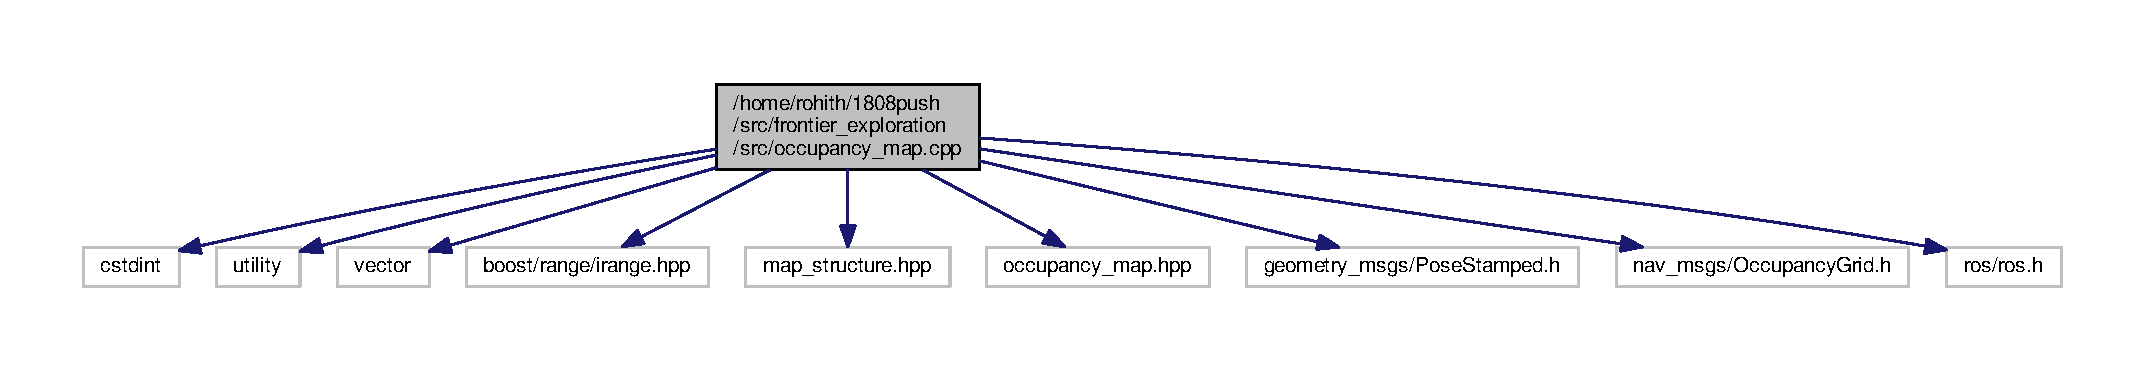
\includegraphics[width=350pt]{occupancy__map_8cpp__incl}
\end{center}
\end{figure}
\subsection*{Variables}
\begin{DoxyCompactItemize}
\item 
const int {\bfseries D\+E\+F\+\_\+\+C\+L\+A\+SS} = -\/255\hypertarget{occupancy__map_8cpp_a42884d7892fcb3d1cd2253fa78ad7eee}{}\label{occupancy__map_8cpp_a42884d7892fcb3d1cd2253fa78ad7eee}

\item 
const int {\bfseries M\+I\+N\+\_\+\+F\+R\+O\+N\+T\+I\+E\+R\+\_\+\+S\+I\+ZE} = 22\hypertarget{occupancy__map_8cpp_a95591e86fc3d599c19ce66d9b073e64d}{}\label{occupancy__map_8cpp_a95591e86fc3d599c19ce66d9b073e64d}

\end{DoxyCompactItemize}


\subsection{Detailed Description}
source file for Occupancy\+Map class 

\begin{DoxyAuthor}{Author}
rohithjayarajan 
\end{DoxyAuthor}
\begin{DoxyDate}{Date}
16/2/2018 
\end{DoxyDate}
\begin{DoxyVersion}{Version}
1.\+1
\end{DoxyVersion}
\hypertarget{occupancy__map__tests_8cpp_DESCRIPTION}{}\subsection{D\+E\+S\+C\+R\+I\+P\+T\+I\+ON}\label{occupancy__map__tests_8cpp_DESCRIPTION}
source file which contains the defintion of Occupancy\+Map class 
\hypertarget{frontier__exploration__node__tests_8cpp}{}\section{/home/rohith/1808push/src/frontier\+\_\+exploration/test/frontier\+\_\+exploration\+\_\+node\+\_\+tests.cpp File Reference}
\label{frontier__exploration__node__tests_8cpp}\index{/home/rohith/1808push/src/frontier\+\_\+exploration/test/frontier\+\_\+exploration\+\_\+node\+\_\+tests.\+cpp@{/home/rohith/1808push/src/frontier\+\_\+exploration/test/frontier\+\_\+exploration\+\_\+node\+\_\+tests.\+cpp}}


source file for testing Map\+Structure class  


{\ttfamily \#include \char`\"{}frontier\+\_\+exploration\+\_\+node.\+hpp\char`\"{}}\\*
{\ttfamily \#include $<$gtest/gtest.\+h$>$}\\*
{\ttfamily \#include $<$cstdint$>$}\\*
{\ttfamily \#include $<$utility$>$}\\*
{\ttfamily \#include $<$vector$>$}\\*
{\ttfamily \#include $<$boost/range/irange.\+hpp$>$}\\*
{\ttfamily \#include \char`\"{}occupancy\+\_\+map.\+hpp\char`\"{}}\\*
{\ttfamily \#include \char`\"{}actionlib/client/simple\+\_\+action\+\_\+client.\+h\char`\"{}}\\*
{\ttfamily \#include \char`\"{}geometry\+\_\+msgs/\+Pose\+Stamped.\+h\char`\"{}}\\*
{\ttfamily \#include \char`\"{}geometry\+\_\+msgs/\+Twist.\+h\char`\"{}}\\*
{\ttfamily \#include \char`\"{}move\+\_\+base\+\_\+msgs/\+Move\+Base\+Action.\+h\char`\"{}}\\*
{\ttfamily \#include \char`\"{}nav\+\_\+msgs/\+Occupancy\+Grid.\+h\char`\"{}}\\*
{\ttfamily \#include \char`\"{}nav\+\_\+msgs/\+Odometry.\+h\char`\"{}}\\*
{\ttfamily \#include \char`\"{}ros/ros.\+h\char`\"{}}\\*
{\ttfamily \#include \char`\"{}tf/transform\+\_\+listener.\+h\char`\"{}}\\*
Include dependency graph for frontier\+\_\+exploration\+\_\+node\+\_\+tests.\+cpp\+:
\nopagebreak
\begin{figure}[H]
\begin{center}
\leavevmode
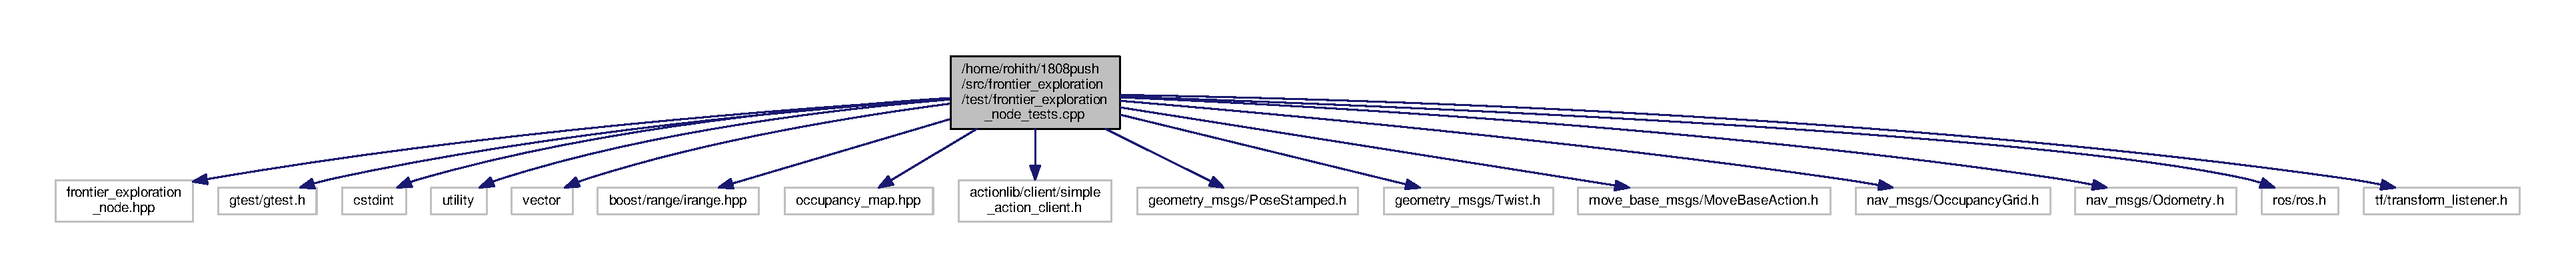
\includegraphics[width=350pt]{frontier__exploration__node__tests_8cpp__incl}
\end{center}
\end{figure}
\subsection*{Classes}
\begin{DoxyCompactItemize}
\item 
class \hyperlink{classPublisherTests}{Publisher\+Tests}
\begin{DoxyCompactList}\small\item\em class \hyperlink{classPublisherTests}{Publisher\+Tests} used for testing publisher \end{DoxyCompactList}\item 
class \hyperlink{classFrontierExploreTests}{Frontier\+Explore\+Tests}
\begin{DoxyCompactList}\small\item\em class \hyperlink{classOccupancyMapTests}{Occupancy\+Map\+Tests} used for setup and teardown for all the tests \end{DoxyCompactList}\end{DoxyCompactItemize}
\subsection*{Functions}
\begin{DoxyCompactItemize}
\item 
\hyperlink{frontier__exploration__node__tests_8cpp_a7b3d1d08f7e936f957443259989e107f}{T\+E\+S\+T\+\_\+F} (\hyperlink{classFrontierExploreTests}{Frontier\+Explore\+Tests}, test\+Pub\+Is\+Okay)
\begin{DoxyCompactList}\small\item\em test function to test publisher for velocity \end{DoxyCompactList}\item 
\hyperlink{frontier__exploration__node__tests_8cpp_af87d07d48ee993f2d6be8bcc4215c3cc}{T\+E\+S\+T\+\_\+F} (\hyperlink{classFrontierExploreTests}{Frontier\+Explore\+Tests}, test\+Map\+Is\+Okay)
\begin{DoxyCompactList}\small\item\em test function to test /map subscription \end{DoxyCompactList}\item 
\hyperlink{frontier__exploration__node__tests_8cpp_a3ed47aec16cf5497b4175f472e110c0b}{T\+E\+S\+T\+\_\+F} (\hyperlink{classFrontierExploreTests}{Frontier\+Explore\+Tests}, test\+Update\+Robot\+Pose)
\begin{DoxyCompactList}\small\item\em test function to test update\+Robot\+Pose method \end{DoxyCompactList}\item 
\hyperlink{frontier__exploration__node__tests_8cpp_a3cda1e232e89bfe191fc93c64dae313e}{T\+E\+S\+T\+\_\+F} (\hyperlink{classFrontierExploreTests}{Frontier\+Explore\+Tests}, test\+Rotate)
\begin{DoxyCompactList}\small\item\em test function to test rotate method \end{DoxyCompactList}\end{DoxyCompactItemize}


\subsection{Detailed Description}
source file for testing Map\+Structure class 

\begin{DoxyAuthor}{Author}
rohithjayarajan 
\end{DoxyAuthor}
\begin{DoxyDate}{Date}
12/15/2018 
\end{DoxyDate}
\begin{DoxyVersion}{Version}
1.\+1
\end{DoxyVersion}
\hypertarget{occupancy__map__tests_8cpp_DESCRIPTION}{}\subsection{D\+E\+S\+C\+R\+I\+P\+T\+I\+ON}\label{occupancy__map__tests_8cpp_DESCRIPTION}
source file which contains tests for Map\+Structure class 

\subsection{Function Documentation}
\index{frontier\+\_\+exploration\+\_\+node\+\_\+tests.\+cpp@{frontier\+\_\+exploration\+\_\+node\+\_\+tests.\+cpp}!T\+E\+S\+T\+\_\+F@{T\+E\+S\+T\+\_\+F}}
\index{T\+E\+S\+T\+\_\+F@{T\+E\+S\+T\+\_\+F}!frontier\+\_\+exploration\+\_\+node\+\_\+tests.\+cpp@{frontier\+\_\+exploration\+\_\+node\+\_\+tests.\+cpp}}
\subsubsection[{\texorpdfstring{T\+E\+S\+T\+\_\+\+F(\+Frontier\+Explore\+Tests, test\+Pub\+Is\+Okay)}{TEST_F(FrontierExploreTests, testPubIsOkay)}}]{\setlength{\rightskip}{0pt plus 5cm}T\+E\+S\+T\+\_\+F (
\begin{DoxyParamCaption}
\item[{{\bf Frontier\+Explore\+Tests}}]{, }
\item[{test\+Pub\+Is\+Okay}]{}
\end{DoxyParamCaption}
)}\hypertarget{frontier__exploration__node__tests_8cpp_a7b3d1d08f7e936f957443259989e107f}{}\label{frontier__exploration__node__tests_8cpp_a7b3d1d08f7e936f957443259989e107f}


test function to test publisher for velocity 


\begin{DoxyParams}{Parameters}
{\em \hyperlink{classFrontierExploreTests}{Frontier\+Explore\+Tests},the} & gtest framework \\
\hline
{\em test\+Pub\+Is\+Okay,the} & name of test \\
\hline
\end{DoxyParams}
\index{frontier\+\_\+exploration\+\_\+node\+\_\+tests.\+cpp@{frontier\+\_\+exploration\+\_\+node\+\_\+tests.\+cpp}!T\+E\+S\+T\+\_\+F@{T\+E\+S\+T\+\_\+F}}
\index{T\+E\+S\+T\+\_\+F@{T\+E\+S\+T\+\_\+F}!frontier\+\_\+exploration\+\_\+node\+\_\+tests.\+cpp@{frontier\+\_\+exploration\+\_\+node\+\_\+tests.\+cpp}}
\subsubsection[{\texorpdfstring{T\+E\+S\+T\+\_\+\+F(\+Frontier\+Explore\+Tests, test\+Map\+Is\+Okay)}{TEST_F(FrontierExploreTests, testMapIsOkay)}}]{\setlength{\rightskip}{0pt plus 5cm}T\+E\+S\+T\+\_\+F (
\begin{DoxyParamCaption}
\item[{{\bf Frontier\+Explore\+Tests}}]{, }
\item[{test\+Map\+Is\+Okay}]{}
\end{DoxyParamCaption}
)}\hypertarget{frontier__exploration__node__tests_8cpp_af87d07d48ee993f2d6be8bcc4215c3cc}{}\label{frontier__exploration__node__tests_8cpp_af87d07d48ee993f2d6be8bcc4215c3cc}


test function to test /map subscription 


\begin{DoxyParams}{Parameters}
{\em \hyperlink{classFrontierExploreTests}{Frontier\+Explore\+Tests},the} & gtest framework \\
\hline
{\em test\+Map\+Is\+Okay,the} & name of test \\
\hline
\end{DoxyParams}
\index{frontier\+\_\+exploration\+\_\+node\+\_\+tests.\+cpp@{frontier\+\_\+exploration\+\_\+node\+\_\+tests.\+cpp}!T\+E\+S\+T\+\_\+F@{T\+E\+S\+T\+\_\+F}}
\index{T\+E\+S\+T\+\_\+F@{T\+E\+S\+T\+\_\+F}!frontier\+\_\+exploration\+\_\+node\+\_\+tests.\+cpp@{frontier\+\_\+exploration\+\_\+node\+\_\+tests.\+cpp}}
\subsubsection[{\texorpdfstring{T\+E\+S\+T\+\_\+\+F(\+Frontier\+Explore\+Tests, test\+Update\+Robot\+Pose)}{TEST_F(FrontierExploreTests, testUpdateRobotPose)}}]{\setlength{\rightskip}{0pt plus 5cm}T\+E\+S\+T\+\_\+F (
\begin{DoxyParamCaption}
\item[{{\bf Frontier\+Explore\+Tests}}]{, }
\item[{test\+Update\+Robot\+Pose}]{}
\end{DoxyParamCaption}
)}\hypertarget{frontier__exploration__node__tests_8cpp_a3ed47aec16cf5497b4175f472e110c0b}{}\label{frontier__exploration__node__tests_8cpp_a3ed47aec16cf5497b4175f472e110c0b}


test function to test update\+Robot\+Pose method 


\begin{DoxyParams}{Parameters}
{\em \hyperlink{classFrontierExploreTests}{Frontier\+Explore\+Tests},the} & gtest framework \\
\hline
{\em test\+Update\+Robot\+Pose,the} & name of test \\
\hline
\end{DoxyParams}
\index{frontier\+\_\+exploration\+\_\+node\+\_\+tests.\+cpp@{frontier\+\_\+exploration\+\_\+node\+\_\+tests.\+cpp}!T\+E\+S\+T\+\_\+F@{T\+E\+S\+T\+\_\+F}}
\index{T\+E\+S\+T\+\_\+F@{T\+E\+S\+T\+\_\+F}!frontier\+\_\+exploration\+\_\+node\+\_\+tests.\+cpp@{frontier\+\_\+exploration\+\_\+node\+\_\+tests.\+cpp}}
\subsubsection[{\texorpdfstring{T\+E\+S\+T\+\_\+\+F(\+Frontier\+Explore\+Tests, test\+Rotate)}{TEST_F(FrontierExploreTests, testRotate)}}]{\setlength{\rightskip}{0pt plus 5cm}T\+E\+S\+T\+\_\+F (
\begin{DoxyParamCaption}
\item[{{\bf Frontier\+Explore\+Tests}}]{, }
\item[{test\+Rotate}]{}
\end{DoxyParamCaption}
)}\hypertarget{frontier__exploration__node__tests_8cpp_a3cda1e232e89bfe191fc93c64dae313e}{}\label{frontier__exploration__node__tests_8cpp_a3cda1e232e89bfe191fc93c64dae313e}


test function to test rotate method 


\begin{DoxyParams}{Parameters}
{\em \hyperlink{classFrontierExploreTests}{Frontier\+Explore\+Tests},the} & gtest framework \\
\hline
{\em test\+Rotate,the} & name of test \\
\hline
\end{DoxyParams}

\hypertarget{map__structure__tests_8cpp}{}\section{/home/rohith/1808push/src/frontier\+\_\+exploration/test/map\+\_\+structure\+\_\+tests.cpp File Reference}
\label{map__structure__tests_8cpp}\index{/home/rohith/1808push/src/frontier\+\_\+exploration/test/map\+\_\+structure\+\_\+tests.\+cpp@{/home/rohith/1808push/src/frontier\+\_\+exploration/test/map\+\_\+structure\+\_\+tests.\+cpp}}


source file for testing Map\+Structure class  


{\ttfamily \#include \char`\"{}map\+\_\+structure.\+hpp\char`\"{}}\\*
{\ttfamily \#include $<$gtest/gtest.\+h$>$}\\*
{\ttfamily \#include $<$cstdint$>$}\\*
{\ttfamily \#include $<$utility$>$}\\*
Include dependency graph for map\+\_\+structure\+\_\+tests.\+cpp\+:
\nopagebreak
\begin{figure}[H]
\begin{center}
\leavevmode
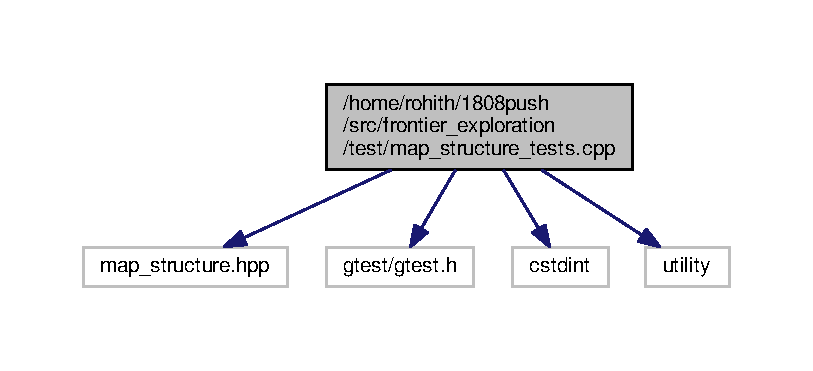
\includegraphics[width=350pt]{map__structure__tests_8cpp__incl}
\end{center}
\end{figure}
\subsection*{Functions}
\begin{DoxyCompactItemize}
\item 
\hyperlink{map__structure__tests_8cpp_a31dc68f3f494ffd101bf6eacccb56e1e}{T\+E\+ST} (Map\+Structure\+Tests, get\+Set\+Is\+On\+Frontier)
\begin{DoxyCompactList}\small\item\em test function to test is\+On\+Frontier variable getter \& setter method Map\+Structure class \end{DoxyCompactList}\item 
\hyperlink{map__structure__tests_8cpp_a9870f5a4123dc5c8228e4bfceec643c5}{T\+E\+ST} (Map\+Structure\+Tests, get\+Setfrontier\+Class)
\begin{DoxyCompactList}\small\item\em test function to test frontier\+Class variable getter \& setter method Map\+Structure class \end{DoxyCompactList}\item 
\hyperlink{map__structure__tests_8cpp_acf1e845e5b15e4a31e680954e21ddd16}{T\+E\+ST} (Map\+Structure\+Tests, get\+Set\+Map\+X\+Y\+Coordinate)
\begin{DoxyCompactList}\small\item\em test function to test x and y variable getter \& setter method Map\+Structure class \end{DoxyCompactList}\item 
\hyperlink{map__structure__tests_8cpp_a4be9751676a0089e376b7e543b8c76ae}{T\+E\+ST} (Map\+Structure\+Tests, get\+Set\+Map\+Data)
\begin{DoxyCompactList}\small\item\em test function to test data variable getter \& setter method Map\+Structure class \end{DoxyCompactList}\end{DoxyCompactItemize}


\subsection{Detailed Description}
source file for testing Map\+Structure class 

\begin{DoxyAuthor}{Author}
rohithjayarajan 
\end{DoxyAuthor}
\begin{DoxyDate}{Date}
12/15/2018 
\end{DoxyDate}
\begin{DoxyVersion}{Version}
1.\+1
\end{DoxyVersion}
\hypertarget{occupancy__map__tests_8cpp_DESCRIPTION}{}\subsection{D\+E\+S\+C\+R\+I\+P\+T\+I\+ON}\label{occupancy__map__tests_8cpp_DESCRIPTION}
source file which contains tests for Map\+Structure class 

\subsection{Function Documentation}
\index{map\+\_\+structure\+\_\+tests.\+cpp@{map\+\_\+structure\+\_\+tests.\+cpp}!T\+E\+ST@{T\+E\+ST}}
\index{T\+E\+ST@{T\+E\+ST}!map\+\_\+structure\+\_\+tests.\+cpp@{map\+\_\+structure\+\_\+tests.\+cpp}}
\subsubsection[{\texorpdfstring{T\+E\+S\+T(\+Map\+Structure\+Tests, get\+Set\+Is\+On\+Frontier)}{TEST(MapStructureTests, getSetIsOnFrontier)}}]{\setlength{\rightskip}{0pt plus 5cm}T\+E\+ST (
\begin{DoxyParamCaption}
\item[{Map\+Structure\+Tests}]{, }
\item[{get\+Set\+Is\+On\+Frontier}]{}
\end{DoxyParamCaption}
)}\hypertarget{map__structure__tests_8cpp_a31dc68f3f494ffd101bf6eacccb56e1e}{}\label{map__structure__tests_8cpp_a31dc68f3f494ffd101bf6eacccb56e1e}


test function to test is\+On\+Frontier variable getter \& setter method Map\+Structure class 


\begin{DoxyParams}{Parameters}
{\em Map\+Structure\+Tests,the} & gtest framework \\
\hline
{\em get\+Set\+Is\+On\+Frontier,the} & name of test \\
\hline
\end{DoxyParams}
\index{map\+\_\+structure\+\_\+tests.\+cpp@{map\+\_\+structure\+\_\+tests.\+cpp}!T\+E\+ST@{T\+E\+ST}}
\index{T\+E\+ST@{T\+E\+ST}!map\+\_\+structure\+\_\+tests.\+cpp@{map\+\_\+structure\+\_\+tests.\+cpp}}
\subsubsection[{\texorpdfstring{T\+E\+S\+T(\+Map\+Structure\+Tests, get\+Setfrontier\+Class)}{TEST(MapStructureTests, getSetfrontierClass)}}]{\setlength{\rightskip}{0pt plus 5cm}T\+E\+ST (
\begin{DoxyParamCaption}
\item[{Map\+Structure\+Tests}]{, }
\item[{get\+Setfrontier\+Class}]{}
\end{DoxyParamCaption}
)}\hypertarget{map__structure__tests_8cpp_a9870f5a4123dc5c8228e4bfceec643c5}{}\label{map__structure__tests_8cpp_a9870f5a4123dc5c8228e4bfceec643c5}


test function to test frontier\+Class variable getter \& setter method Map\+Structure class 


\begin{DoxyParams}{Parameters}
{\em Map\+Structure\+Tests,the} & gtest framework \\
\hline
{\em get\+Setfrontier\+Class,the} & name of test \\
\hline
\end{DoxyParams}
\index{map\+\_\+structure\+\_\+tests.\+cpp@{map\+\_\+structure\+\_\+tests.\+cpp}!T\+E\+ST@{T\+E\+ST}}
\index{T\+E\+ST@{T\+E\+ST}!map\+\_\+structure\+\_\+tests.\+cpp@{map\+\_\+structure\+\_\+tests.\+cpp}}
\subsubsection[{\texorpdfstring{T\+E\+S\+T(\+Map\+Structure\+Tests, get\+Set\+Map\+X\+Y\+Coordinate)}{TEST(MapStructureTests, getSetMapXYCoordinate)}}]{\setlength{\rightskip}{0pt plus 5cm}T\+E\+ST (
\begin{DoxyParamCaption}
\item[{Map\+Structure\+Tests}]{, }
\item[{get\+Set\+Map\+X\+Y\+Coordinate}]{}
\end{DoxyParamCaption}
)}\hypertarget{map__structure__tests_8cpp_acf1e845e5b15e4a31e680954e21ddd16}{}\label{map__structure__tests_8cpp_acf1e845e5b15e4a31e680954e21ddd16}


test function to test x and y variable getter \& setter method Map\+Structure class 


\begin{DoxyParams}{Parameters}
{\em Map\+Structure\+Tests,the} & gtest framework \\
\hline
{\em get\+Set\+Map\+X\+Y\+Coordinate,the} & name of test \\
\hline
\end{DoxyParams}
\index{map\+\_\+structure\+\_\+tests.\+cpp@{map\+\_\+structure\+\_\+tests.\+cpp}!T\+E\+ST@{T\+E\+ST}}
\index{T\+E\+ST@{T\+E\+ST}!map\+\_\+structure\+\_\+tests.\+cpp@{map\+\_\+structure\+\_\+tests.\+cpp}}
\subsubsection[{\texorpdfstring{T\+E\+S\+T(\+Map\+Structure\+Tests, get\+Set\+Map\+Data)}{TEST(MapStructureTests, getSetMapData)}}]{\setlength{\rightskip}{0pt plus 5cm}T\+E\+ST (
\begin{DoxyParamCaption}
\item[{Map\+Structure\+Tests}]{, }
\item[{get\+Set\+Map\+Data}]{}
\end{DoxyParamCaption}
)}\hypertarget{map__structure__tests_8cpp_a4be9751676a0089e376b7e543b8c76ae}{}\label{map__structure__tests_8cpp_a4be9751676a0089e376b7e543b8c76ae}


test function to test data variable getter \& setter method Map\+Structure class 


\begin{DoxyParams}{Parameters}
{\em Map\+Structure\+Tests,the} & gtest framework \\
\hline
{\em get\+Set\+Map\+Data,the} & name of test \\
\hline
\end{DoxyParams}

\hypertarget{occupancy__map__tests_8cpp}{}\section{/home/rohith/1808push/src/frontier\+\_\+exploration/test/occupancy\+\_\+map\+\_\+tests.cpp File Reference}
\label{occupancy__map__tests_8cpp}\index{/home/rohith/1808push/src/frontier\+\_\+exploration/test/occupancy\+\_\+map\+\_\+tests.\+cpp@{/home/rohith/1808push/src/frontier\+\_\+exploration/test/occupancy\+\_\+map\+\_\+tests.\+cpp}}


source file for testing Occupancy\+Map class  


{\ttfamily \#include $<$gtest/gtest.\+h$>$}\\*
{\ttfamily \#include $<$cstdint$>$}\\*
{\ttfamily \#include $<$utility$>$}\\*
{\ttfamily \#include $<$vector$>$}\\*
{\ttfamily \#include $<$boost/range/irange.\+hpp$>$}\\*
{\ttfamily \#include \char`\"{}map\+\_\+structure.\+hpp\char`\"{}}\\*
{\ttfamily \#include \char`\"{}occupancy\+\_\+map.\+hpp\char`\"{}}\\*
{\ttfamily \#include \char`\"{}geometry\+\_\+msgs/\+Pose\+Stamped.\+h\char`\"{}}\\*
{\ttfamily \#include \char`\"{}nav\+\_\+msgs/\+Occupancy\+Grid.\+h\char`\"{}}\\*
{\ttfamily \#include \char`\"{}ros/ros.\+h\char`\"{}}\\*
Include dependency graph for occupancy\+\_\+map\+\_\+tests.\+cpp\+:
\nopagebreak
\begin{figure}[H]
\begin{center}
\leavevmode
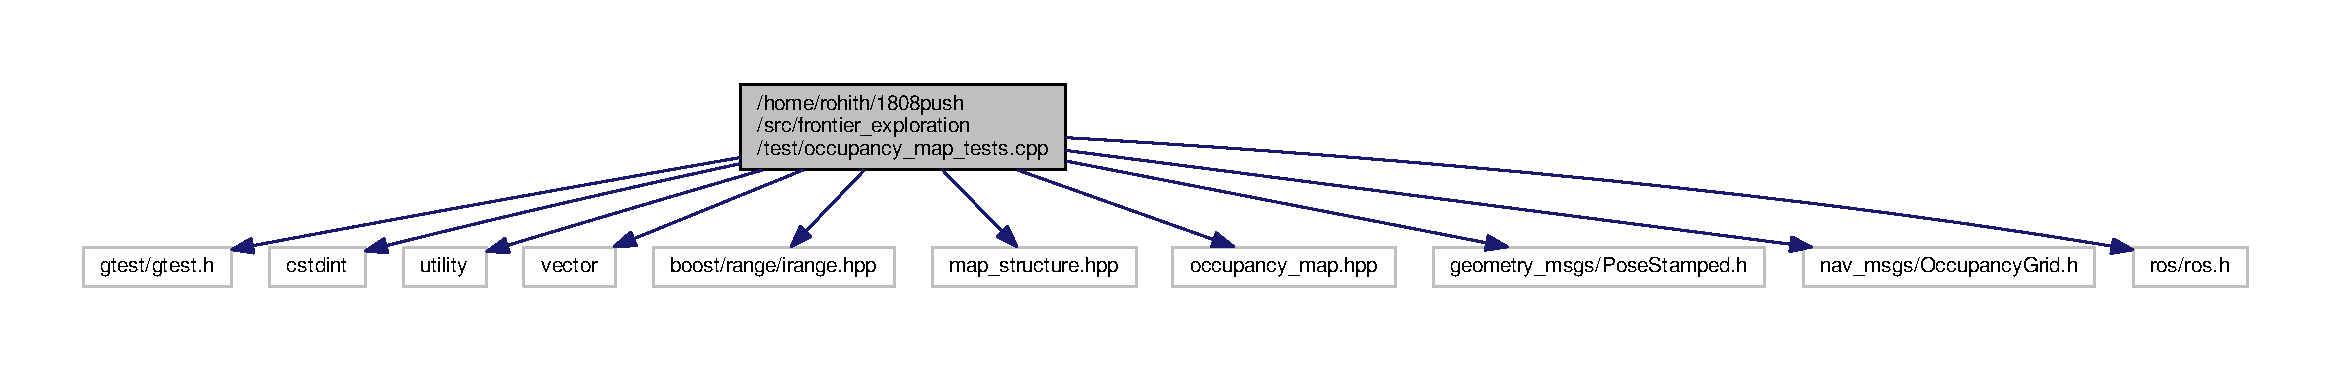
\includegraphics[width=350pt]{occupancy__map__tests_8cpp__incl}
\end{center}
\end{figure}
\subsection*{Classes}
\begin{DoxyCompactItemize}
\item 
class \hyperlink{classOccupancyMapTests}{Occupancy\+Map\+Tests}
\begin{DoxyCompactList}\small\item\em class \hyperlink{classOccupancyMapTests}{Occupancy\+Map\+Tests} used for setup and teardown for all the tests \end{DoxyCompactList}\end{DoxyCompactItemize}
\subsection*{Functions}
\begin{DoxyCompactItemize}
\item 
\hyperlink{occupancy__map__tests_8cpp_aaed26bc70cef776c08924a0c46de2e21}{T\+E\+S\+T\+\_\+F} (\hyperlink{classOccupancyMapTests}{Occupancy\+Map\+Tests}, get\+Set\+Map\+Reslution)
\begin{DoxyCompactList}\small\item\em test function to test resolution variable getter \& setter method Occupancy\+Map class \end{DoxyCompactList}\item 
\hyperlink{occupancy__map__tests_8cpp_a8b9696cd259bde480c72d50817d674b1}{T\+E\+S\+T\+\_\+F} (\hyperlink{classOccupancyMapTests}{Occupancy\+Map\+Tests}, get\+Set\+Map\+Height)
\begin{DoxyCompactList}\small\item\em test function to test height variable getter \& setter method Occupancy\+Map class \end{DoxyCompactList}\item 
\hyperlink{occupancy__map__tests_8cpp_a8a26fe87f9433f839ec8b9b59dcb34fd}{T\+E\+S\+T\+\_\+F} (\hyperlink{classOccupancyMapTests}{Occupancy\+Map\+Tests}, get\+Set\+Map\+Width)
\begin{DoxyCompactList}\small\item\em test function to test width variable getter \& setter method Occupancy\+Map class \end{DoxyCompactList}\item 
\hyperlink{occupancy__map__tests_8cpp_a00b1a37310df622280211e7b865f9609}{T\+E\+S\+T\+\_\+F} (\hyperlink{classOccupancyMapTests}{Occupancy\+Map\+Tests}, get\+Set\+Map\+Oigin)
\begin{DoxyCompactList}\small\item\em test function to test origin variable getter \& setter method Occupancy\+Map class \end{DoxyCompactList}\item 
\hyperlink{occupancy__map__tests_8cpp_a78aa146a5cfad52fb0dc750000125731}{T\+E\+S\+T\+\_\+F} (\hyperlink{classOccupancyMapTests}{Occupancy\+Map\+Tests}, test\+Is\+Frontier)
\begin{DoxyCompactList}\small\item\em test function to test is\+Frontier method Occupancy\+Map class \end{DoxyCompactList}\item 
\hyperlink{occupancy__map__tests_8cpp_a1029ad624defc57a8207a45aa2eb2f0d}{T\+E\+S\+T\+\_\+F} (\hyperlink{classOccupancyMapTests}{Occupancy\+Map\+Tests}, test\+Classify\+Frontiers)
\begin{DoxyCompactList}\small\item\em test function to test classify\+Frontiers method Occupancy\+Map class \end{DoxyCompactList}\item 
\hyperlink{occupancy__map__tests_8cpp_ae5e3fb60e709e757f1211026c5c95e58}{T\+E\+S\+T\+\_\+F} (\hyperlink{classOccupancyMapTests}{Occupancy\+Map\+Tests}, test\+Frontier\+Centroid)
\begin{DoxyCompactList}\small\item\em test function to test get\+Frontier\+Centroid method Occupancy\+Map class \end{DoxyCompactList}\item 
\hyperlink{occupancy__map__tests_8cpp_a1544a2a9ceeb62fd58dd8ce9d3eba540}{T\+E\+S\+T\+\_\+F} (\hyperlink{classOccupancyMapTests}{Occupancy\+Map\+Tests}, test\+Grid2world)
\begin{DoxyCompactList}\small\item\em test function to test grid2world method Occupancy\+Map class \end{DoxyCompactList}\item 
\hyperlink{occupancy__map__tests_8cpp_a5188f97411144d62e660933c0b310b3d}{T\+E\+S\+T\+\_\+F} (\hyperlink{classOccupancyMapTests}{Occupancy\+Map\+Tests}, test\+Detect\+Frontiers\+Center\+World)
\begin{DoxyCompactList}\small\item\em test function to test detect\+Frontiers\+Center\+World method Occupancy\+Map class \end{DoxyCompactList}\item 
\hyperlink{occupancy__map__tests_8cpp_ab5ac6991e479b745caec21f6f267c2b7}{T\+E\+S\+T\+\_\+F} (\hyperlink{classOccupancyMapTests}{Occupancy\+Map\+Tests}, test\+Read\+Occupancy\+Grid)
\begin{DoxyCompactList}\small\item\em test function to test read\+Occupancy\+Grid method Occupancy\+Map class \end{DoxyCompactList}\end{DoxyCompactItemize}


\subsection{Detailed Description}
source file for testing Occupancy\+Map class 

\begin{DoxyAuthor}{Author}
rohithjayarajan 
\end{DoxyAuthor}
\begin{DoxyDate}{Date}
12/15/2018 
\end{DoxyDate}
\begin{DoxyVersion}{Version}
0.\+1
\end{DoxyVersion}
\hypertarget{occupancy__map__tests_8cpp_DESCRIPTION}{}\subsection{D\+E\+S\+C\+R\+I\+P\+T\+I\+ON}\label{occupancy__map__tests_8cpp_DESCRIPTION}
source file which contains tests for Occupancy\+Map class 

\subsection{Function Documentation}
\index{occupancy\+\_\+map\+\_\+tests.\+cpp@{occupancy\+\_\+map\+\_\+tests.\+cpp}!T\+E\+S\+T\+\_\+F@{T\+E\+S\+T\+\_\+F}}
\index{T\+E\+S\+T\+\_\+F@{T\+E\+S\+T\+\_\+F}!occupancy\+\_\+map\+\_\+tests.\+cpp@{occupancy\+\_\+map\+\_\+tests.\+cpp}}
\subsubsection[{\texorpdfstring{T\+E\+S\+T\+\_\+\+F(\+Occupancy\+Map\+Tests, get\+Set\+Map\+Reslution)}{TEST_F(OccupancyMapTests, getSetMapReslution)}}]{\setlength{\rightskip}{0pt plus 5cm}T\+E\+S\+T\+\_\+F (
\begin{DoxyParamCaption}
\item[{{\bf Occupancy\+Map\+Tests}}]{, }
\item[{get\+Set\+Map\+Reslution}]{}
\end{DoxyParamCaption}
)}\hypertarget{occupancy__map__tests_8cpp_aaed26bc70cef776c08924a0c46de2e21}{}\label{occupancy__map__tests_8cpp_aaed26bc70cef776c08924a0c46de2e21}


test function to test resolution variable getter \& setter method Occupancy\+Map class 


\begin{DoxyParams}{Parameters}
{\em \hyperlink{classOccupancyMapTests}{Occupancy\+Map\+Tests},the} & gtest framework \\
\hline
{\em get\+Set\+Map\+Reslution,the} & name of test \\
\hline
\end{DoxyParams}
\index{occupancy\+\_\+map\+\_\+tests.\+cpp@{occupancy\+\_\+map\+\_\+tests.\+cpp}!T\+E\+S\+T\+\_\+F@{T\+E\+S\+T\+\_\+F}}
\index{T\+E\+S\+T\+\_\+F@{T\+E\+S\+T\+\_\+F}!occupancy\+\_\+map\+\_\+tests.\+cpp@{occupancy\+\_\+map\+\_\+tests.\+cpp}}
\subsubsection[{\texorpdfstring{T\+E\+S\+T\+\_\+\+F(\+Occupancy\+Map\+Tests, get\+Set\+Map\+Height)}{TEST_F(OccupancyMapTests, getSetMapHeight)}}]{\setlength{\rightskip}{0pt plus 5cm}T\+E\+S\+T\+\_\+F (
\begin{DoxyParamCaption}
\item[{{\bf Occupancy\+Map\+Tests}}]{, }
\item[{get\+Set\+Map\+Height}]{}
\end{DoxyParamCaption}
)}\hypertarget{occupancy__map__tests_8cpp_a8b9696cd259bde480c72d50817d674b1}{}\label{occupancy__map__tests_8cpp_a8b9696cd259bde480c72d50817d674b1}


test function to test height variable getter \& setter method Occupancy\+Map class 


\begin{DoxyParams}{Parameters}
{\em \hyperlink{classOccupancyMapTests}{Occupancy\+Map\+Tests},the} & gtest framework \\
\hline
{\em get\+Set\+Map\+Height,the} & name of test \\
\hline
\end{DoxyParams}
\index{occupancy\+\_\+map\+\_\+tests.\+cpp@{occupancy\+\_\+map\+\_\+tests.\+cpp}!T\+E\+S\+T\+\_\+F@{T\+E\+S\+T\+\_\+F}}
\index{T\+E\+S\+T\+\_\+F@{T\+E\+S\+T\+\_\+F}!occupancy\+\_\+map\+\_\+tests.\+cpp@{occupancy\+\_\+map\+\_\+tests.\+cpp}}
\subsubsection[{\texorpdfstring{T\+E\+S\+T\+\_\+\+F(\+Occupancy\+Map\+Tests, get\+Set\+Map\+Width)}{TEST_F(OccupancyMapTests, getSetMapWidth)}}]{\setlength{\rightskip}{0pt plus 5cm}T\+E\+S\+T\+\_\+F (
\begin{DoxyParamCaption}
\item[{{\bf Occupancy\+Map\+Tests}}]{, }
\item[{get\+Set\+Map\+Width}]{}
\end{DoxyParamCaption}
)}\hypertarget{occupancy__map__tests_8cpp_a8a26fe87f9433f839ec8b9b59dcb34fd}{}\label{occupancy__map__tests_8cpp_a8a26fe87f9433f839ec8b9b59dcb34fd}


test function to test width variable getter \& setter method Occupancy\+Map class 


\begin{DoxyParams}{Parameters}
{\em \hyperlink{classOccupancyMapTests}{Occupancy\+Map\+Tests},the} & gtest framework \\
\hline
{\em get\+Set\+Map\+Width,the} & name of test \\
\hline
\end{DoxyParams}
\index{occupancy\+\_\+map\+\_\+tests.\+cpp@{occupancy\+\_\+map\+\_\+tests.\+cpp}!T\+E\+S\+T\+\_\+F@{T\+E\+S\+T\+\_\+F}}
\index{T\+E\+S\+T\+\_\+F@{T\+E\+S\+T\+\_\+F}!occupancy\+\_\+map\+\_\+tests.\+cpp@{occupancy\+\_\+map\+\_\+tests.\+cpp}}
\subsubsection[{\texorpdfstring{T\+E\+S\+T\+\_\+\+F(\+Occupancy\+Map\+Tests, get\+Set\+Map\+Oigin)}{TEST_F(OccupancyMapTests, getSetMapOigin)}}]{\setlength{\rightskip}{0pt plus 5cm}T\+E\+S\+T\+\_\+F (
\begin{DoxyParamCaption}
\item[{{\bf Occupancy\+Map\+Tests}}]{, }
\item[{get\+Set\+Map\+Oigin}]{}
\end{DoxyParamCaption}
)}\hypertarget{occupancy__map__tests_8cpp_a00b1a37310df622280211e7b865f9609}{}\label{occupancy__map__tests_8cpp_a00b1a37310df622280211e7b865f9609}


test function to test origin variable getter \& setter method Occupancy\+Map class 


\begin{DoxyParams}{Parameters}
{\em \hyperlink{classOccupancyMapTests}{Occupancy\+Map\+Tests},the} & gtest framework \\
\hline
{\em get\+Set\+Map\+Metadata,the} & name of test \\
\hline
\end{DoxyParams}
\index{occupancy\+\_\+map\+\_\+tests.\+cpp@{occupancy\+\_\+map\+\_\+tests.\+cpp}!T\+E\+S\+T\+\_\+F@{T\+E\+S\+T\+\_\+F}}
\index{T\+E\+S\+T\+\_\+F@{T\+E\+S\+T\+\_\+F}!occupancy\+\_\+map\+\_\+tests.\+cpp@{occupancy\+\_\+map\+\_\+tests.\+cpp}}
\subsubsection[{\texorpdfstring{T\+E\+S\+T\+\_\+\+F(\+Occupancy\+Map\+Tests, test\+Is\+Frontier)}{TEST_F(OccupancyMapTests, testIsFrontier)}}]{\setlength{\rightskip}{0pt plus 5cm}T\+E\+S\+T\+\_\+F (
\begin{DoxyParamCaption}
\item[{{\bf Occupancy\+Map\+Tests}}]{, }
\item[{test\+Is\+Frontier}]{}
\end{DoxyParamCaption}
)}\hypertarget{occupancy__map__tests_8cpp_a78aa146a5cfad52fb0dc750000125731}{}\label{occupancy__map__tests_8cpp_a78aa146a5cfad52fb0dc750000125731}


test function to test is\+Frontier method Occupancy\+Map class 


\begin{DoxyParams}{Parameters}
{\em \hyperlink{classOccupancyMapTests}{Occupancy\+Map\+Tests},the} & gtest framework \\
\hline
{\em get\+Set\+Map\+Metadata,the} & name of test \\
\hline
\end{DoxyParams}
\index{occupancy\+\_\+map\+\_\+tests.\+cpp@{occupancy\+\_\+map\+\_\+tests.\+cpp}!T\+E\+S\+T\+\_\+F@{T\+E\+S\+T\+\_\+F}}
\index{T\+E\+S\+T\+\_\+F@{T\+E\+S\+T\+\_\+F}!occupancy\+\_\+map\+\_\+tests.\+cpp@{occupancy\+\_\+map\+\_\+tests.\+cpp}}
\subsubsection[{\texorpdfstring{T\+E\+S\+T\+\_\+\+F(\+Occupancy\+Map\+Tests, test\+Classify\+Frontiers)}{TEST_F(OccupancyMapTests, testClassifyFrontiers)}}]{\setlength{\rightskip}{0pt plus 5cm}T\+E\+S\+T\+\_\+F (
\begin{DoxyParamCaption}
\item[{{\bf Occupancy\+Map\+Tests}}]{, }
\item[{test\+Classify\+Frontiers}]{}
\end{DoxyParamCaption}
)}\hypertarget{occupancy__map__tests_8cpp_a1029ad624defc57a8207a45aa2eb2f0d}{}\label{occupancy__map__tests_8cpp_a1029ad624defc57a8207a45aa2eb2f0d}


test function to test classify\+Frontiers method Occupancy\+Map class 


\begin{DoxyParams}{Parameters}
{\em \hyperlink{classOccupancyMapTests}{Occupancy\+Map\+Tests},the} & gtest framework \\
\hline
{\em get\+Set\+Map\+Metadata,the} & name of test \\
\hline
\end{DoxyParams}
\index{occupancy\+\_\+map\+\_\+tests.\+cpp@{occupancy\+\_\+map\+\_\+tests.\+cpp}!T\+E\+S\+T\+\_\+F@{T\+E\+S\+T\+\_\+F}}
\index{T\+E\+S\+T\+\_\+F@{T\+E\+S\+T\+\_\+F}!occupancy\+\_\+map\+\_\+tests.\+cpp@{occupancy\+\_\+map\+\_\+tests.\+cpp}}
\subsubsection[{\texorpdfstring{T\+E\+S\+T\+\_\+\+F(\+Occupancy\+Map\+Tests, test\+Frontier\+Centroid)}{TEST_F(OccupancyMapTests, testFrontierCentroid)}}]{\setlength{\rightskip}{0pt plus 5cm}T\+E\+S\+T\+\_\+F (
\begin{DoxyParamCaption}
\item[{{\bf Occupancy\+Map\+Tests}}]{, }
\item[{test\+Frontier\+Centroid}]{}
\end{DoxyParamCaption}
)}\hypertarget{occupancy__map__tests_8cpp_ae5e3fb60e709e757f1211026c5c95e58}{}\label{occupancy__map__tests_8cpp_ae5e3fb60e709e757f1211026c5c95e58}


test function to test get\+Frontier\+Centroid method Occupancy\+Map class 


\begin{DoxyParams}{Parameters}
{\em \hyperlink{classOccupancyMapTests}{Occupancy\+Map\+Tests},the} & gtest framework \\
\hline
{\em get\+Set\+Map\+Metadata,the} & name of test \\
\hline
\end{DoxyParams}
\index{occupancy\+\_\+map\+\_\+tests.\+cpp@{occupancy\+\_\+map\+\_\+tests.\+cpp}!T\+E\+S\+T\+\_\+F@{T\+E\+S\+T\+\_\+F}}
\index{T\+E\+S\+T\+\_\+F@{T\+E\+S\+T\+\_\+F}!occupancy\+\_\+map\+\_\+tests.\+cpp@{occupancy\+\_\+map\+\_\+tests.\+cpp}}
\subsubsection[{\texorpdfstring{T\+E\+S\+T\+\_\+\+F(\+Occupancy\+Map\+Tests, test\+Grid2world)}{TEST_F(OccupancyMapTests, testGrid2world)}}]{\setlength{\rightskip}{0pt plus 5cm}T\+E\+S\+T\+\_\+F (
\begin{DoxyParamCaption}
\item[{{\bf Occupancy\+Map\+Tests}}]{, }
\item[{test\+Grid2world}]{}
\end{DoxyParamCaption}
)}\hypertarget{occupancy__map__tests_8cpp_a1544a2a9ceeb62fd58dd8ce9d3eba540}{}\label{occupancy__map__tests_8cpp_a1544a2a9ceeb62fd58dd8ce9d3eba540}


test function to test grid2world method Occupancy\+Map class 


\begin{DoxyParams}{Parameters}
{\em \hyperlink{classOccupancyMapTests}{Occupancy\+Map\+Tests},the} & gtest framework \\
\hline
{\em get\+Set\+Map\+Metadata,the} & name of test \\
\hline
\end{DoxyParams}
\index{occupancy\+\_\+map\+\_\+tests.\+cpp@{occupancy\+\_\+map\+\_\+tests.\+cpp}!T\+E\+S\+T\+\_\+F@{T\+E\+S\+T\+\_\+F}}
\index{T\+E\+S\+T\+\_\+F@{T\+E\+S\+T\+\_\+F}!occupancy\+\_\+map\+\_\+tests.\+cpp@{occupancy\+\_\+map\+\_\+tests.\+cpp}}
\subsubsection[{\texorpdfstring{T\+E\+S\+T\+\_\+\+F(\+Occupancy\+Map\+Tests, test\+Detect\+Frontiers\+Center\+World)}{TEST_F(OccupancyMapTests, testDetectFrontiersCenterWorld)}}]{\setlength{\rightskip}{0pt plus 5cm}T\+E\+S\+T\+\_\+F (
\begin{DoxyParamCaption}
\item[{{\bf Occupancy\+Map\+Tests}}]{, }
\item[{test\+Detect\+Frontiers\+Center\+World}]{}
\end{DoxyParamCaption}
)}\hypertarget{occupancy__map__tests_8cpp_a5188f97411144d62e660933c0b310b3d}{}\label{occupancy__map__tests_8cpp_a5188f97411144d62e660933c0b310b3d}


test function to test detect\+Frontiers\+Center\+World method Occupancy\+Map class 


\begin{DoxyParams}{Parameters}
{\em \hyperlink{classOccupancyMapTests}{Occupancy\+Map\+Tests},the} & gtest framework \\
\hline
{\em get\+Set\+Map\+Metadata,the} & name of test \\
\hline
\end{DoxyParams}
\index{occupancy\+\_\+map\+\_\+tests.\+cpp@{occupancy\+\_\+map\+\_\+tests.\+cpp}!T\+E\+S\+T\+\_\+F@{T\+E\+S\+T\+\_\+F}}
\index{T\+E\+S\+T\+\_\+F@{T\+E\+S\+T\+\_\+F}!occupancy\+\_\+map\+\_\+tests.\+cpp@{occupancy\+\_\+map\+\_\+tests.\+cpp}}
\subsubsection[{\texorpdfstring{T\+E\+S\+T\+\_\+\+F(\+Occupancy\+Map\+Tests, test\+Read\+Occupancy\+Grid)}{TEST_F(OccupancyMapTests, testReadOccupancyGrid)}}]{\setlength{\rightskip}{0pt plus 5cm}T\+E\+S\+T\+\_\+F (
\begin{DoxyParamCaption}
\item[{{\bf Occupancy\+Map\+Tests}}]{, }
\item[{test\+Read\+Occupancy\+Grid}]{}
\end{DoxyParamCaption}
)}\hypertarget{occupancy__map__tests_8cpp_ab5ac6991e479b745caec21f6f267c2b7}{}\label{occupancy__map__tests_8cpp_ab5ac6991e479b745caec21f6f267c2b7}


test function to test read\+Occupancy\+Grid method Occupancy\+Map class 


\begin{DoxyParams}{Parameters}
{\em \hyperlink{classOccupancyMapTests}{Occupancy\+Map\+Tests},the} & gtest framework \\
\hline
{\em test\+Read\+Occupancy\+Grid,the} & name of test \\
\hline
\end{DoxyParams}

%--- End generated contents ---

% Index
\backmatter
\newpage
\phantomsection
\clearemptydoublepage
\addcontentsline{toc}{chapter}{Index}
\printindex

\end{document}
